\documentclass[12pt, a4paper]{article}\usepackage[]{graphicx}\usepackage[]{color}
%% maxwidth is the original width if it is less than linewidth
%% otherwise use linewidth (to make sure the graphics do not exceed the margin)
\makeatletter
\def\maxwidth{ %
  \ifdim\Gin@nat@width>\linewidth
    \linewidth
  \else
    \Gin@nat@width
  \fi
}
\makeatother

\definecolor{fgcolor}{rgb}{0.345, 0.345, 0.345}
\newcommand{\hlnum}[1]{\textcolor[rgb]{0.686,0.059,0.569}{#1}}%
\newcommand{\hlstr}[1]{\textcolor[rgb]{0.192,0.494,0.8}{#1}}%
\newcommand{\hlcom}[1]{\textcolor[rgb]{0.678,0.584,0.686}{\textit{#1}}}%
\newcommand{\hlopt}[1]{\textcolor[rgb]{0,0,0}{#1}}%
\newcommand{\hlstd}[1]{\textcolor[rgb]{0.345,0.345,0.345}{#1}}%
\newcommand{\hlkwa}[1]{\textcolor[rgb]{0.161,0.373,0.58}{\textbf{#1}}}%
\newcommand{\hlkwb}[1]{\textcolor[rgb]{0.69,0.353,0.396}{#1}}%
\newcommand{\hlkwc}[1]{\textcolor[rgb]{0.333,0.667,0.333}{#1}}%
\newcommand{\hlkwd}[1]{\textcolor[rgb]{0.737,0.353,0.396}{\textbf{#1}}}%
\let\hlipl\hlkwb

\usepackage{framed}
\makeatletter
\newenvironment{kframe}{%
 \def\at@end@of@kframe{}%
 \ifinner\ifhmode%
  \def\at@end@of@kframe{\end{minipage}}%
  \begin{minipage}{\columnwidth}%
 \fi\fi%
 \def\FrameCommand##1{\hskip\@totalleftmargin \hskip-\fboxsep
 \colorbox{shadecolor}{##1}\hskip-\fboxsep
     % There is no \\@totalrightmargin, so:
     \hskip-\linewidth \hskip-\@totalleftmargin \hskip\columnwidth}%
 \MakeFramed {\advance\hsize-\width
   \@totalleftmargin\z@ \linewidth\hsize
   \@setminipage}}%
 {\par\unskip\endMakeFramed%
 \at@end@of@kframe}
\makeatother

\definecolor{shadecolor}{rgb}{.97, .97, .97}
\definecolor{messagecolor}{rgb}{0, 0, 0}
\definecolor{warningcolor}{rgb}{1, 0, 1}
\definecolor{errorcolor}{rgb}{1, 0, 0}
\newenvironment{knitrout}{}{} % an empty environment to be redefined in TeX

\usepackage{alltt}

%%%%%%%%%%%%%%%%%%%%%%%%%%%%%%%%%%%%%%%%%%%%%%%%%%%%%%%%%%%%%%%%
% LaTeX packages
%\usepackage[OT4]{polski}
\usepackage[cp1250]{inputenc}
\usepackage[top=2.5cm, bottom=2.5cm, left=2cm, right=2cm]{geometry}
\usepackage{graphicx}
\usepackage{float}
\usepackage[colorlinks=true, linkcolor=blue]{hyperref}


%%%%%%%%%%%%%%%%%%%%%%%%%%%%%%%%%%%%%%%%%%%%%%%%%%%%%%%%%%%%%%%%
% global settings


\IfFileExists{upquote.sty}{\usepackage{upquote}}{}
\begin{document}

%%%%%%%%%%%%%%%%%%%%%%%%%%%%%%%%%%%%%%%%%%%%%%%%%%%%%%%%%%%%%%%%
% title page
\title{Estimation theory -- report template}
\author{Name and surname \\ Student no.}
\maketitle
\tableofcontents 


%%%%%%%%%%%%%%%%%%%%%%%%%%%%%%%%%%%%%%%%%%%%%%%%%%%%%%%%%%%%%%%%
\section{Exercise 1}

In order to include R code chunk  use the following syntax:
\begin{knitrout}
\definecolor{shadecolor}{rgb}{0.969, 0.969, 0.969}\color{fgcolor}\begin{kframe}
\begin{alltt}
\hlcom{# random sample from standard normal distribution}
\hlstd{X} \hlkwb{<-} \hlkwd{rnorm}\hlstd{(}\hlnum{100}\hlstd{)}

\hlcom{# summary statistics}
\hlkwd{summary}\hlstd{(X)}
\end{alltt}
\begin{verbatim}
##     Min.  1st Qu.   Median     Mean  3rd Qu.     Max. 
## -2.50700 -0.64010  0.06037  0.05680  0.70220  2.15400
\end{verbatim}
\end{kframe}
\end{knitrout}

Remark: To display the output of a code chunk but not the underlying R code, you specify the echo=FALSE option.

%%%%%%%%%%%%%%%%%%%%%%%%%%%%%%%%%%%%%%%%%%%%%%%%%%%%%%%%%%%%%%%%
\section{Exercise 2}

R code chunks can  be used to create plots dynamically too.
For example,  to obtain histogram write:
\begin{knitrout}
\definecolor{shadecolor}{rgb}{0.969, 0.969, 0.969}\color{fgcolor}\begin{kframe}
\begin{alltt}
\hlkwd{hist}\hlstd{(X,} \hlkwc{main}\hlstd{=}\hlstr{"Histogram"}\hlstd{)}
\end{alltt}
\end{kframe}\begin{figure}[H]

{\centering 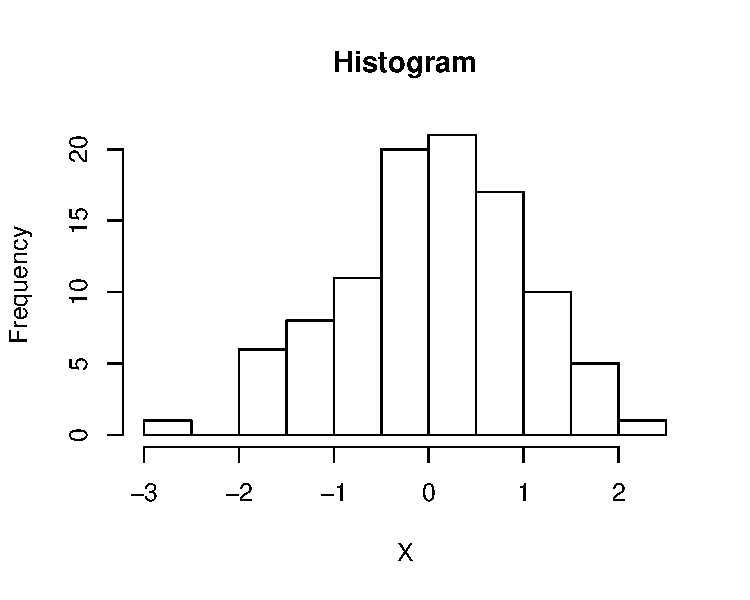
\includegraphics[width=\maxwidth]{figure/example_hist-1} 

}

\caption[Add caption here]{Add caption here}\label{fig:example_hist}
\end{figure}


\end{knitrout}
Note that one can easily add  reference to the generated figures.  For example: Figure~\ref{fig:example_hist} shows histogram.


Creating nice looking tables is not much more difficult. For this purpose you can use
function {\em xtable()}. Here is a small example:
% latex table generated in R 3.2.3 by xtable 1.8-2 package
% Mon Oct 16 11:46:21 2017
\begin{table}[H]
\centering
\begin{tabular}{rrrrrr}
  \hline
 & 1 & 2 & 3 & 4 & 5 \\ 
  \hline
1 & 0.319 & -0.317 & 0.185 & 0.432 & 0.400 \\ 
  2 & 1.763 & 1.779 & -0.665 & -0.142 & -0.956 \\ 
  3 & 0.652 & 0.206 & -0.394 & -0.907 & -1.288 \\ 
  4 & -0.731 & -1.508 & -0.134 & -0.306 & -0.226 \\ 
   \hline
\end{tabular}
\caption{Add caption here} 
\label{tab:table1}
\end{table}

You can add a reference to our table~\ref{tab:table1} too.


%%%%%%%%%%%%%%%%%%%%%%%%%%%%%%%%%%%%%%%%%%%%%%%%%%%%%%%%%%%%%%%%
\section{Exercise 3}

If needed (e.g. when answering theoretical problems etc.), use \LaTeX \ syntax to add mathematical formulas. For example, inline (within text) formulas can be included using: $a^2+b^2=c^2$. On the other hand, 	displayed equations can be added as follows:
\begin{equation}
\label{eq:wzor1}
\overline{X} = \frac{1}{n}\sum_{i=1}^n X_i,
\end{equation}
where $n$ denotes sample size.


%%%%%%%%%%%%%%%%%%%%%%%%%%%%%%%%%%%%%%%%%%%%%%%%%%%%%%%%%%%%%%%%
\section{Exercise 4}

{\bf A few final suggestions:}
\begin{itemize}
\item The results of simulations or analysis should be presented in a clear format.
\item When you plot the graphs, remember about axis descriptions, setting appropriate axis limits (e.g: \verb+ plot (..., xlim = c (x.min, x.max), ylim = c (y.min, y.max)+), adding legend (necessary when there are several lines in the graph), and adding a caption under the graph or table.
\item If possible try to show the results in a condensed form (e.g. comparing several charts in one figure, comparing the results in a single table, etc.).

\item It is worth to consider whether all R-codes should be visible in the report (option {\verb+ echo = TRUE / FALSE+}).

\item Remember to carefully format the R-codes and write appropriate comments (also in the case of chunks that are invisible in the report. You can use the following option available in RStudio: $Code \; \rightarrow\; Reformate \;  Code$.
\end{itemize}

%%%%%%%%%%%%%%%%%%%%%%%%%%%%%%%%%%%%%%%%%%%%%%%%%%%%%%%%%%%%%%%%
When using additional source materials (books, links, etc.)
do not forget to include appropriate references.  For example, let us assume 
we want to cite Dalgard (2008). Then the bibliography section should contain:

\begin{thebibliography}{}
 
\bibitem{Dalgard2008}
  Peter Dalgaard, \emph{Introductory Statistics with R}, Springer-Verlag New York, 2008.

\end{thebibliography}

\end{document}
